\section{Company description}\label{sec:company}
Allseas Engineering B.V. is a Dutch company that specializes in offshore pipeline
installation and subsea construction. The company was founded in 1985 by Edward Heerema
and is headquartered in Delft, the Netherlands. Allseas is known for its innovative
engineering solutions and state-of-the-art vessels, such as the Pioneering Spirit,
which is the largest construction vessel in the world.
The company has a global presence with offices in the Netherlands, Switzerland,
and the United Kingdom, and employs over 2,500 people worldwide.

Allseas' core business is the installation of subsea pipelines and the
construction of offshore structures for the oil and gas industry. The company's
vessels are equipped with advanced technology and equipment to perform a wide
range of offshore operations. \cite{allseas}

Allseas' direct clients are other other engineering firms in this industry or governments. For instance, developing countries may hire Allseas to build infrastructure for oil and gas transportation. The company's indirect clients are the end-users of the infrastructure, such as oil and gas companies or inhibitants of the country. In the remainder of this report the term "stakesholders" will be used to refer to both direct and indirect clients. It should be mentioned that Allseas is an independently run company, meaning it has no investors and allows it to make decisions based on its own interests.

Allseas' organizational structure is divided into several departments, which
are shown in Figure \ref{fig:allseas_org}.
\begin{figure}[H]
    \centering
    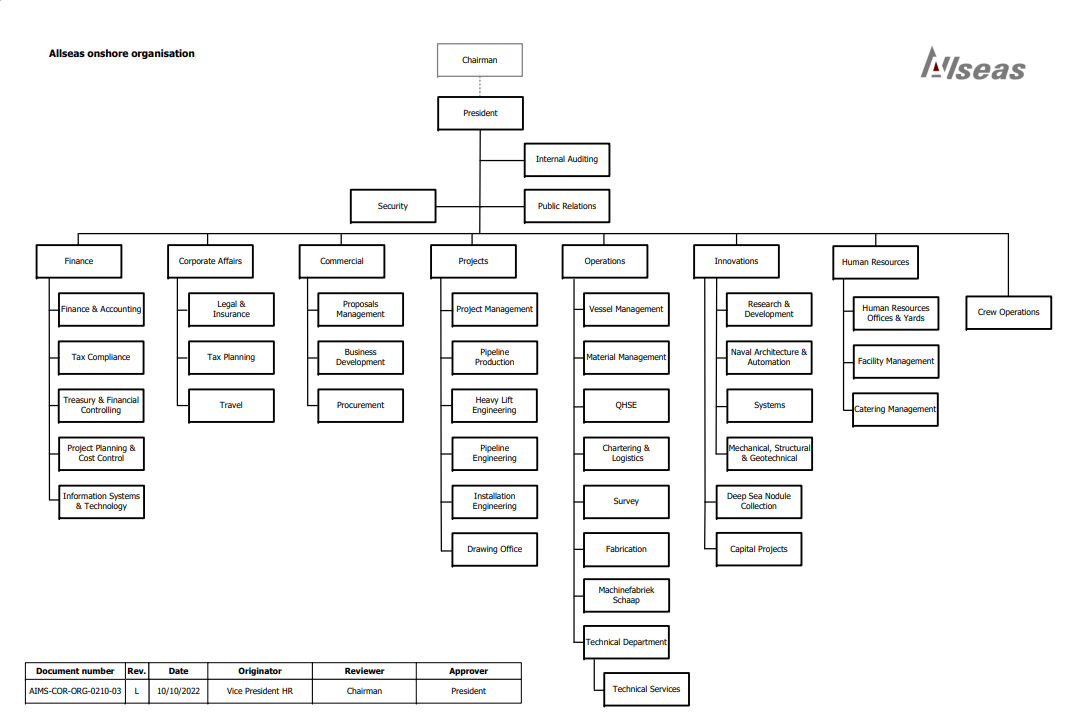
\includegraphics[width=\textwidth]{images/allseas_organisation.png}
    \caption{Allseas organizational structure.}
    \label{fig:allseas_org}
\end{figure}

The company's innovations department is responsible for the design and
development of new technologies and solutions to improve the efficiency and
safety of offshore operations. It is in this department that the internship
project is situated. Figure \ref{fig:allseas_innovations} shows the
organizational structure of the innovations department. In particular, the
project is performed in the sub-department of Research \& Development Delft,
which is led by the department manager (Dominik Bujakiewicz). The project is
supervised by the senior R\&D engineer (J. Ramlakhan) and performed by the
intern (Philip Soliman).
\begin{figure}[H]
    \centering
    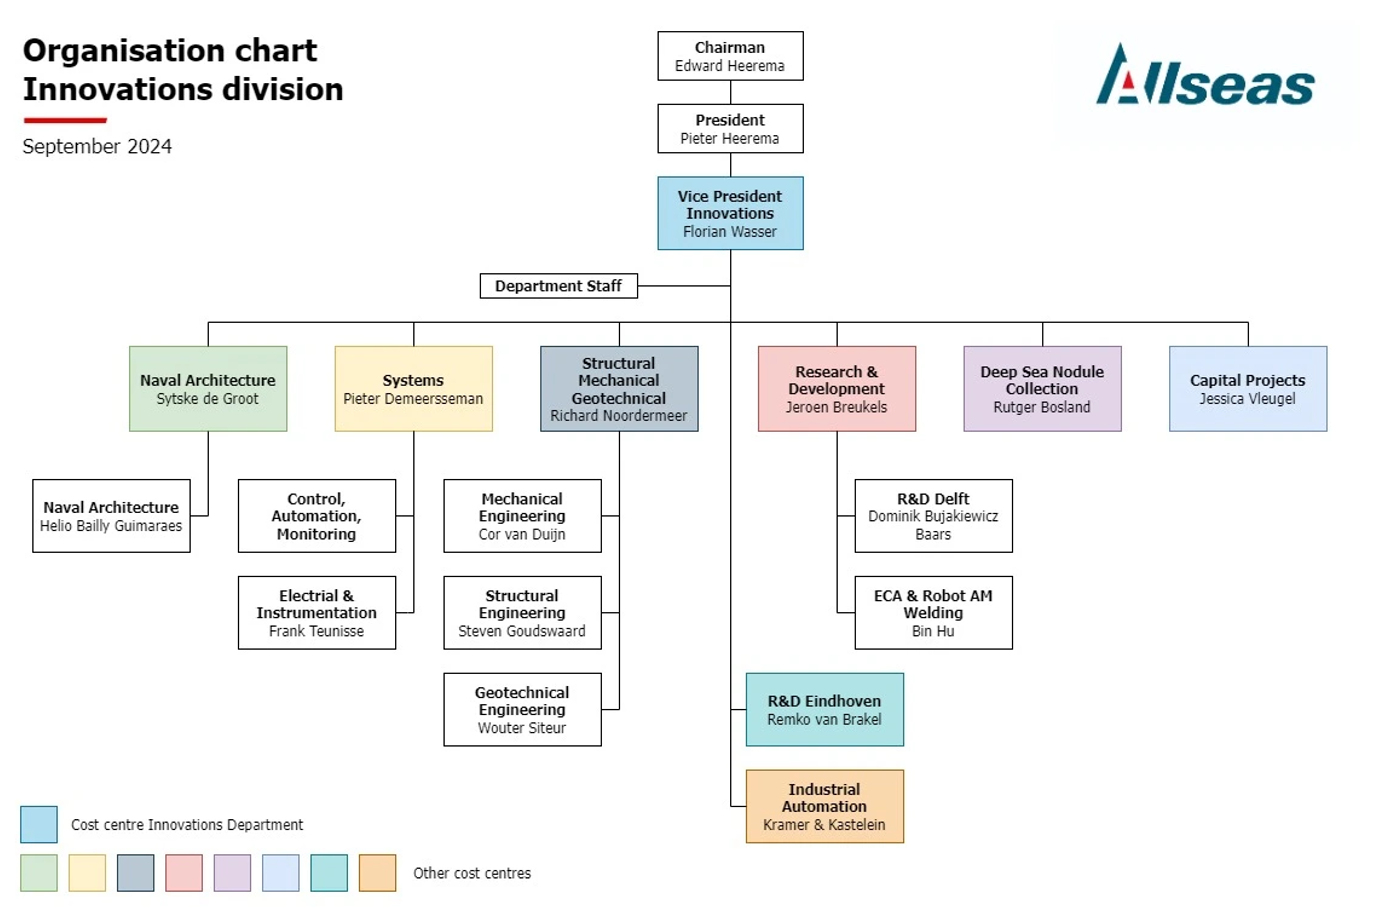
\includegraphics[width=\textwidth]{images/allseas_innovations_dep.png}
    \caption{Allseas innovations department organizational structure.}
    \label{fig:allseas_innovations}
\end{figure}
